\section{Particle Kinematics}

\subsection{Position, velocity, acceleration}
\blue{Complete in  "Position, velocity, and acceleration"}\\
\red{Add the table summary shown in Fig \ref{fig:PosVelAcce}}

\begin{figure}[h!]
    \centering
    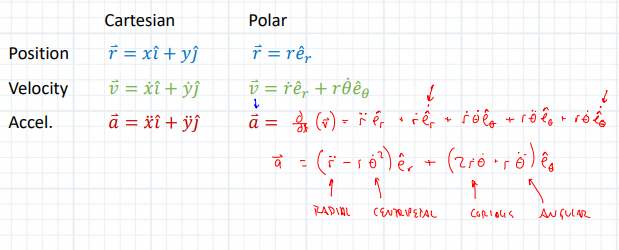
\includegraphics[width=0.9\textwidth]{ParticleKinematicsFigs/PosVelAcce.png}
    \caption{From L07-Notes, slide 2}
    \label{fig:PosVelAcce}
\end{figure}

    \subsubsection{Graphical understanding}
    \blue{Complete in reference page "Position, velocity, and acceleration"} \\

\subsection{Rotating frames}
    \subsubsection{Angular velocity}
    \blue{Complete in reference page "Rotations and angular velocity"} \\
    \subsubsection{Angular acceleration}
        \blue{Complete in reference page "Position, velocity, and acceleration"} \\
        \red{This equation is displayed under the title "Velocity and acceleration in polar basis". Add the description of each term as shown in Fig \ref{fig:AngularAccelerationEq}}
    \begin{figure}[h!]
        \centering   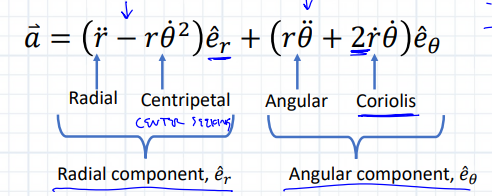
\includegraphics[width=0.6\textwidth]{ParticleKinematicsFigs/AngularAcceleration.png}
        \caption{From L08-Notes, Slide 2}
        \label{fig:AngularAccelerationEq}
    \end{figure}
    
\subsection{Tangential}
    \subsubsection{Normal basis}
    \blue{Complete in reference page "Tangential/normal basis"} \\
    \subsubsection{Normal and Tangential acceleration}
        \blue{Complete in reference page "Tangential/normal basis"} \\
    \subsubsection{Curvature}
        \blue{Complete in reference page "Tangential/normal basis"} \\

\subsection{\red{System comparison: Cartesian/Polar/Tangent-Normal}}
\red{Add summary table as in Fig \ref{fig:SystemsComparison}}

\begin{figure} [h!]
    \centering
    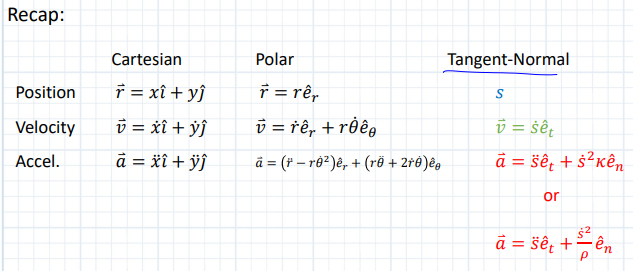
\includegraphics[width=0.9\textwidth]{ParticleKinematicsFigs/SystemsComparison.png}
    \caption{From L12-Notes, slide 3}
    \label{fig:SystemsComparison}
\end{figure}

\subsection{\red{Applications}}
    \subsubsection{\red{Train wheels}}
    \red{This was mentioned in lecture but it was not expanded. It would be a great idea to include a picture or example.} Refers to "angular velocity".
    
    \subsubsection{\red{Variable inertia flywheel}}
    \red{This is mentioned in L07-Notes, Slide 6. This paper is cited \url{https://doi.org/10.1016/j.egyr.2020.01.001}. This picture is included \ref{fig:AppFlywheel}.} Refers to "Angular accelerations".
    \begin{figure}[h!]
        \centering
        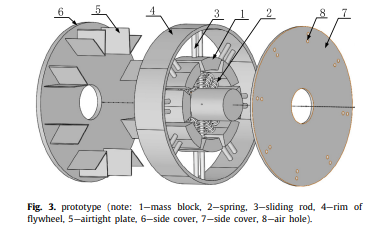
\includegraphics{ParticleKinematicsFigs/AppFlywheel.png}
        \caption{From L07-Notes, slide 6.}
        \label{fig:AppFlywheel}
    \end{figure}
    
    \subsubsection{Celestial velocities}
    \blue{Complete in "Celestial Velocities".} Refers to "angular velocity" and "angular acceleration".
    
    \subsubsection{Track transition curves}
    \blue{Complete in "Track transition curves".} Refers to "position, velocity, and acceleration" and "Tangential".

    \subsubsection{\red{Roller coaster}}
    \red{This topic needs to be created, it was mentioned in lecture with no information or figure}